\documentclass[conference]{IEEEtran}
\IEEEoverridecommandlockouts
% The preceding line is only needed to identify funding in the first footnote. If that is unneeded, please comment it out.
\usepackage{cite}
\usepackage{amsmath,amssymb,amsfonts}
\usepackage{algorithmic}
\usepackage{graphicx}
\usepackage{textcomp}
\usepackage{xcolor}

\usepackage{listings}

\def\BibTeX{{\rm B\kern-.05em{\sc i\kern-.025em b}\kern-.08em
    T\kern-.1667em\lower.7ex\hbox{E}\kern-.125emX}}

% --- Definizione del linguaggio Solidity ---
\lstdefinelanguage{Solidity}{
  morekeywords={
    pragma, solidity, contract, library, interface, struct, event, modifier, function, returns,
    if, else, for, while, do, break, continue, return, emit, revert, require, assert,
    mapping, memory, storage, calldata, public, private, internal, external, view, pure, payable,
    address, bool, string, bytes, uint, uint8, uint16, uint32, uint64, uint128, uint256,
    int, int8, int16, int32, int64, int128, int256,
    new, delete, this, super, msg, block, tx
  },
  sensitive=true,
  morecomment=[l]{//},     % Commenti singola linea
  morecomment=[s]{/*}{*/}, % Commenti multilinea
  morestring=[b]",         % Stringhe tra doppi apici
  morestring=[b]'          % Stringhe tra apici singoli
}

\definecolor{codegreen}{rgb}{0,0.6,0}
\definecolor{codegray}{rgb}{0.5,0.5,0.5}
\definecolor{codepurple}{rgb}{0.58,0,0.82}
\definecolor{backcolour}{rgb}{0.95,0.95,0.92}
% --- Doom One Light Color Definitions ---
% (Add this to your preamble)
\definecolor{doomBack}{RGB}{250, 250, 250}     % #fafafa
\definecolor{doomComment}{RGB}{156, 156, 156}   % #9c9c9c
\definecolor{doomKeyword}{RGB}{198, 120, 221}   % #c678dd (Purple/Magenta)
\definecolor{doomString}{RGB}{152, 195, 121}    % #98c379 (Green)
\definecolor{doomNumber}{RGB}{209, 154, 102}    % #d19a66 (Orange)
\definecolor{doomDefault}{RGB}{77, 77, 77}      % #4d4d4d (Default Text)
% Setup section. -----------------------------------|


\lstdefinestyle{soliditystyle}{
  language=Solidity,
  basicstyle=\ttfamily\small,
  backgroundcolor=\color{doomBack}, 
  commentstyle=\color{doomComment},
  keywordstyle=\color{doomKeyword},
  numberstyle=\tiny\color{doomNumber},
  stringstyle=\color{doomString},
  basicstyle=\ttfamily\footnotesize\color{doomDefault},
  breakatwhitespace=false,         
  breaklines=true,                 
  captionpos=b,                    
  keepspaces=true,                 
  numbers=left,                    
  numbersep=8pt,                  
  showspaces=false,                
  showstringspaces=false,
  showtabs=false,                  
  tabsize=2
}

\begin{document}

% Designing and Developing a Token-Driven NFT Marketplace on Ethereum
% Design and Implementation of a Token-Based NFT Marketplace on Ethereum
\title{Design and Implementation of a Token-NFT-Liquidity Smart Contract Suite\\
%{\footnotesize \textsuperscript{*}Note: Sub-titles are not captured in Xplore and
%should not be used}
%\thanks{Identify applicable funding agency here. If none, delete this.}
}

\author{\IEEEauthorblockN{1\textsuperscript{st} Luca Sforza}
\IEEEauthorblockA{
sforza.2050030@studenti.uniroma1.it}
\and
\IEEEauthorblockN{2\textsuperscript{nd} Roberto Di Rosa}
\IEEEauthorblockA{
dirosa.2043388@studenti.uniroma1.it, }
}

\maketitle

\begin{abstract}
Smart contracts allow the creation of applications that run on the blockchain.
We aim to present a suite of smart contracts designed to manage NFT (Non-Fungible Token) auctions using a custom token called SapiCoin.
We have deployed the auction on the blockchain
that utilizes SapiCoin, and to obtain SapiCoin in order 
to participate in the auction, 
we have created a Liquidity Pool that enables the exchange of Ether for SapiCoin.
\end{abstract}

\section{Introduction}

From a programming perspective, Smart Contracts can be seen as classes in traditional programming languages such as Java.

To create a Token, one must therefore define a class that represents the Token and manages transactions involving that currency.

Other smart contracts (e.g., an auction) can use Tokens as a means of payment within the contract itself.

However, to avoid binding a smart contract to a specific Token and to promote code reusability, the concept of a Token can be abstracted.

The Ethereum community standardized this abstraction through a document known as ERC-20. % TODO: reference

A Token is therefore represented by an Interface (a concept similar to those found in other programming languages).

A smart contract that aims to function as a Token must extend this interface and implement its methods.

The same concept is applied to NFTs, standardized through ERC-721. % TODO: reference

In contrast, there is no community standard for auctions, so the design of such smart contracts must be created from scratch.

% TODO: parla della liquidity pool

\section{Token}

ERC-20 è lo standard che rappresenta un token nelle blockchain EVM compatibili.

Non esiste una figura centrale che possono emmettere questi standard, ma community come Etherum Magician
, permettono di discutere di miglioramenti dello standard Ethereum tramite IEA % TODO: reference

Lo standard impone che un token è uno smart contract con
determinati metodi implementati.

\subsection{Polimorfismo dell'EVM}

Per fare questo si necessita del polimorfismo.

Nell'Ethereum Virtual Machine non esistono istruzioni per gestire classi astratte, ma la VM stessa è poliformica.

Quando si chiama un metodo di uno smart contract tramite una transazione, per accedere
all'indirizzo di memoria del metodo si esegue l'hash della segnatura della funzione. % reference

Nel caso il metodo chiamato non esiste allora viene chiamata una funzione di fallback di default
(che può essere sovrascritta).

Grazie a questo funzionamento dell'EVM è possibile implementare
un qualsiasi standard.

Se volessimio implementare un contratto che gestisce un asta di NFTs
allora esso chiamerà le funzioni che hanno l'hash della signatura come quelle 
definite dallo standard ERC-20.

\subsection{Design of the standard ERC-20}

Uno smart contract lo possiamo visualizzare come una classe.

Linguaggi di programmazione come solidity permettono
di rappresentare l'idea di Interfaccia. Quindi possiamo vicolare uno smart
contract ad avedere i metodi imposti dallo standard eredidando i metodi astratti
di un interfaccia come mostrato in Fig. \ref{code:erc20}.

Ovviamente questo è puro zucchero sintattico poiché la EVM stessa è già poliformica
, infatti l'erederietà può essere omessa.

\begin{figure}
\centering
\begin{lstlisting}[style=soliditystyle]
    contract SapiCoin is ERC20 {
        /* implementation */
    }
\end{lstlisting}
\caption{Polimorfism on Solidity} % TODO: inglese sbagliato
\label{code:erc20}
\end{figure}


\begin{figure}[htbp]
\centerline{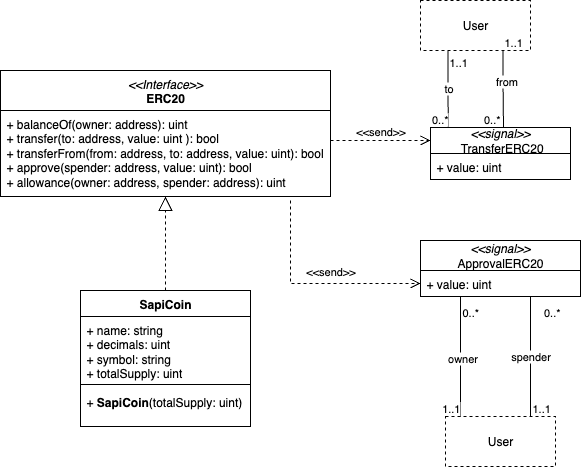
\includegraphics[width=0.35\textwidth]{token.png}}
\caption{UML Class Diagram of a Token.}
\label{uml:token}
\end{figure}

In Figura \ref{uml:token} è possibile vedere un overview dello standard ERC-20.

Lo standard ERC-20 impone per un token di implementare i seguenti metodi:

\begin{enumerate}
    \item \textbf{balanceOf(address owner)} ritorna la quantità di token che un certo address possiede
    \item \textbf{transfer(address to, uint256 value)} permette di inviare dei token verso un determinato address (parametro \texttt{to}).
    \item \textbf{approve(address spender, uint256 value)} permette ad un address (lo \texttt{spender}) di poter spendere una certa quantà di token che possiede l'address che invia la trasazione.
    \item \textbf{transferFrom(address from, address to, uint256 value)} permette di trasferire da un certo address (owner dei token) (non necesssariamente quello che esegue la trasazione)
    verso un altro address una determinata quantità di token specificata in \texttt{value}. Chiaramente non deve essere possibile a chi non ha diritto di spendere i nostri token, infatti
    chi esegue la trasazione deve essere stato approvato (tramite il metodo approve) di poterla eseguire.
    \item \textbf{allowance(address owner, address spender)} permette di sapere quanti token un \texttt{owner} ha approvato verso uno \texttt{spender}.
\end{enumerate}

Tutto il sistema di approve è molto utile da un punto di vista programmatico.

Noi utenti possiamo chiamare approve verso un certo smart contract per una determinata quantità di token.

Cos'i uno smart contract può usare i nostri token per offrire un servizio.

ERC-20 offre anche un insieme da eventi che un token dovrebbe emettere quando cambia lo stato interno del contratto, così le operazioni
avvenute in uno smart contract possono essere rintracciate e visualizzati da applicazioni front-end come etherscan. % TODO: link etherscan

\subsection{Eventi}

Nella figura \ref{uml:token} sono descritti i vari eventi emessi un modo asincrono dall'ERC-20, in particolare:

\begin{enumerate}
    \item Transfer che traccia i trasferimenti di token tra utenti.
    \item Approval che traccia le approvazioni da owner a spender.
\end{enumerate}

In Solidity esiste un costrutto per rappresentare questi eventi come mostrato in Fig. \ref{code:events}.

\begin{figure}
\centering
\begin{lstlisting}[style=soliditystyle]
    event Transfer(address indexed _from, address indexed _to, uint256 _value);
    event Approval(address indexed _owner, address indexed _spender, uint256 _value);
\end{lstlisting}
\caption{Events on Solidity} % TODO: inglese sbagliato
\label{code:events}
\end{figure}

\subsection{Implementazione SapiCoin}

Per implementare uno specifico Token, nel nostro caso SapiCoin, non è presente
una logica extra oltre ad essere un token. Se volessimo implementare uno stablecoin oppure un wrapped coin dovremmo
aggiungere metodi per gestire lo scambio del token con la vera valuta che rappresenta (per esempio USDT o WETH).

L'implementazione delle altre funzionalità standard di un token è facilmente reperibile online (in alcuni casi sono embedded in ambienti di sviluppo soldity).

L'unica cosa modificata sono le vanità del token, ovvero il nome del token, la quantità di decimali che il token possiede (nel nostro caso 18 decimali) e il simbolo del token (SAC).

Avendo messo 18 decimali la quantità più piccola di SapiCoin che è possibile ottenere è $1 \cdot 10^{-18}$.

Però esendo solo una vanità, a basso livello abbiamo accesso solo ad un numero intero unsigned da 256 bit.

Quindi ad esempio 4 SapiCoin in memoria è salvato come $4 \cdot 10^{18}$.

\section{NFTs}

\begin{figure}[htbp]
\centerline{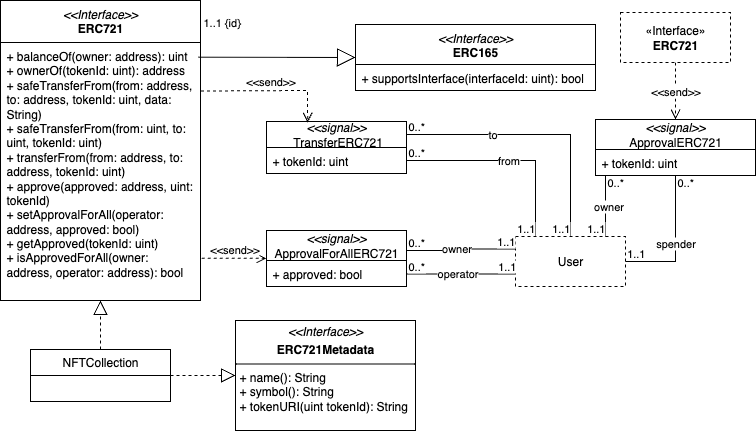
\includegraphics[width=0.5\textwidth]{nft.png}}
\caption{UML Class Diagram of a NFT.}
\label{uml:nft}
\end{figure}


Secondo lo standard very ERC-721 compliant contract must implement the ERC721 and ERC165 interfaces come mostrato in figura
\ref{uml:nft}. % TODO: reference https://eips.ethereum.org/EIPS/eip-721

\subsection{Standard ERC-165}
Lo standard ERC-165 definisce un meccanismo per dichiarare e verificare se un contratto implementa una determinata interfaccia.  
In altre parole, serve per permettere ad altri contratti di interrogare un contratto e capire se supporta una certa funzionalità (ad esempio ERC-721, ERC-20, ecc.).

\textbf{supportsInterface(bytes4 interfaceID)}:  
    permette di verificare se il contratto implementa l'interfaccia identificata da \texttt{interfaceID}.  
    Restituisce \texttt{true} se l'interfaccia è supportata e \texttt{false} altrimenti.  

\subsection{Standard ERC-721}
L'interfaccia ERC-721 definisce lo standard per i NFT. 
Ogni token è unico e distinto, a differenza degli ERC-20 che sono fungibili (tutti uguali).  
Le funzioni da implementare sono:

\begin{enumerate}
    \item \textbf{balanceOf(address owner)}:  
    restituisce il numero di NFT posseduti da un determinato indirizzo.  

    \item \textbf{ownerOf(uint256 tokenId)}:  
    restituisce l'indirizzo del proprietario del token identificato da \texttt{tokenId}.  

    \item \textbf{safeTransferFrom(address from, address to, uint256 tokenId, bytes data)}:  
    trasferisce in modo sicuro la proprietà di un NFT da un indirizzo a un altro.  
    Se il destinatario è un contratto, viene chiamata la funzione \texttt{onERC721Received} per verificare che possa ricevere NFT.
    Per gli scopi di questo progetto abbiamo ignorato questo caso e per il contratto \texttt{auction} non abbiamo implementato la funzione \texttt{onERC721Received}.
    Genera un errore se:
    \begin{itemize}
        \item \texttt{msg.sender} non è il proprietario o un operatore autorizzato;
        \item \texttt{from} non è l'attuale proprietario;
        \item \texttt{to} è lo zero address;
        \item il token non esiste.
    \end{itemize}

    \item \textbf{safeTransferFrom(address from, address to, uint256 tokenId)}:  
    identica alla funzione precedente, ma senza il parametro aggiuntivo \texttt{data} (che viene impostato a stringa vuota).

    \item \textbf{transferFrom(address from, address to, uint256 tokenId)}:  
    trasferisce la proprietà di un NFT senza effettuare controlli aggiuntivi sulla capacità del destinatario di riceverlo.  
    È responsabilità del chiamante assicurarsi che \texttt{to} sia in grado di gestire NFT.  
    Genera errore nelle stesse condizioni di \texttt{safeTransferFrom}.

    \item \textbf{approve(address approved, uint256 tokenId)}:  
    consente al proprietario di approvare un altro indirizzo (\texttt{approved}) per trasferire il token specificato (\texttt{tokenId}).  
    Se viene passato l'indirizzo zero, rimuove ogni approvazione esistente.

    \item \textbf{setApprovalForAll(address operator, bool approved)}:  
    permette a un utente di abilitare o disabilitare un operatore che può gestire tutti i suoi NFT.  
    Genera l'evento \texttt{ApprovalForAll} e consente di avere più operatori per lo stesso proprietario.

    \item \textbf{getApproved(uint256 tokenId)}:  
    restituisce l'indirizzo approvato per la gestione di un determinato token.  
    Se non esiste alcun indirizzo approvato, restituisce lo zero address.  
    Genera errore se il token non è valido.

    \item \textbf{isApprovedForAll(address owner, address operator)}:  
    verifica se un operatore è stato approvato per gestire tutti i token di un determinato proprietario.  
    Restituisce \texttt{true} se è autorizzato, \texttt{false} altrimenti.
\end{enumerate}

Come ERC-20 i contratti che implementano ERC-721 dovrebbero emettere i seguenti eventi:

\begin{enumerate}
    \item \textbf{Transfer(address indexed from, address indexed to, uint256 indexed tokenId)}:  
    viene emesso ogni volta che la proprietà di un NFT cambia, sia in caso di trasferimento, creazione (\texttt{from == 0}) o distruzione (\texttt{to == 0}).  
    Quando un trasferimento avviene, l'eventuale indirizzo approvato per quel token viene automaticamente azzerato.

    \item \textbf{Approval(address indexed owner, address indexed approved, uint256 indexed tokenId)}:  
    viene emesso quando viene impostato o rimosso un indirizzo approvato per un NFT specifico.  
    L'indirizzo zero indica che non esiste più un indirizzo approvato per quel token.

    \item \textbf{ApprovalForAll(address indexed owner, address indexed operator, bool approved)}:  
    viene emesso quando un proprietario abilita o disabilita un operatore che può gestire tutti i suoi NFT.  
    L'operatore può quindi effettuare trasferimenti o approvazioni per conto del proprietario.
\end{enumerate}

\subsection{Metadata e vanità opzionali}

Estendere l'interfaccia \texttt{ERC721Metadata} non è obbligatorio
per lo standard ERC-721, serve unicamente per aggiungere vanità ai NFT.

Grazie a questa interfaccia possiamo ottenere il nome della collezione NFT, il simbolo della collezione e
tramite il metodo \textbf{tokenURI(uint256 tokenId)} possiamo ottenere URL associato all'NFT.

Questo link può essere verso l'immagine che NFT rappresenta o altre informazioni.

% TODO: verificare cosa fa veramente Ferrari
Per esempio Ferrari crea un NFT per una macchina venduta, quindi potrebbero implementare questa interfaccia per la loro collezione NFT
per dare in output un link ad una pagina internet dove sono salvate tutte le informazioni della macchina.

Dipende molto dalle funzionalità che vogliamo incorporare nel nostro NFT, ma l'archiettura dietro agli NFT rimane sempre la stessa.

Infatti anche per lo standard ERC-721 come per lo standard ERC-20 possiamo trovare tantissime implementazioni da riusare per la nostra collezione.

Per lo scopo di questo progetto abbiamo creato un NFT per l'immagine \ref{img:pepe}.

\begin{figure}[htbp]
\centerline{
\includegraphics[width=0.3\textwidth]{image_nft.png}}
\caption{Imagine associata all'NFT che abbiamo fatto il minting}
\label{img:pepe}
\end{figure}

\section{Auction}

Non esiste uno standard per le auction di NFT, quindi per crearne una bisogna occorrere ad altre strategie.

Per esempio si può utilizzare un sistema di auction con i contratti già deployati sulla blockchain
e creare un asta tramite quel sistema. Cos'i ogni utente del sistema può accedere alla tua asta, per esempio OpenSea % TODO: reference

Oppure creare lo smart contract a mano dell'asta e fare il deploy nella blockchain.

Per il secondo approccio abbiamo lo svantaggio che non abbiamo un applicazione front-end dove è possibile
usufruire del servizio. Ma quello che si può fare è pubblicare il contratto su etherscan cosi collegando un Wallet (come Metamask)
si può interaggire con lo smart contract tramite web browser.

Purtroppo i principali marketplace di NFT hanno tolto il loro supporto sulle blockchain di test, quindi
abbiamo optato ad implemntarla da zero.

\subsection{Design of Auction}

\begin{figure}[htbp]
\centerline{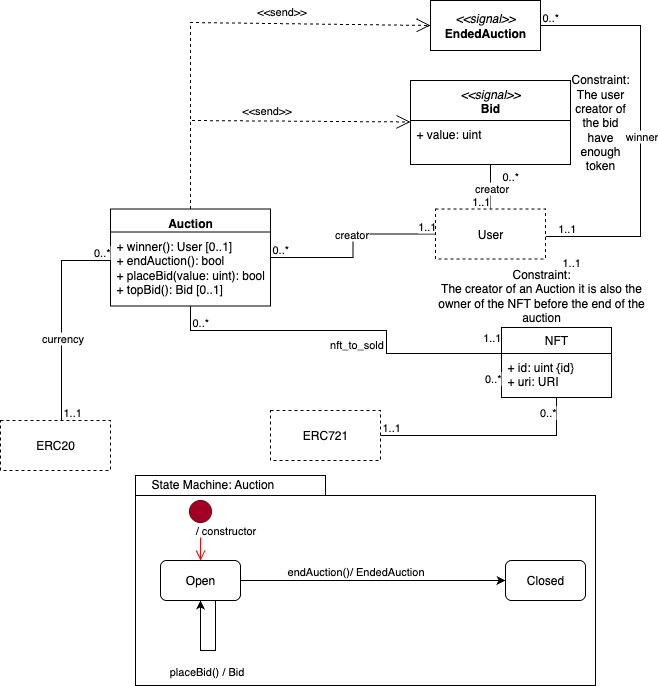
\includegraphics[width=0.5\textwidth]{auction.png}}
\caption{UML of a Auction}
\label{uml:auction}
\end{figure}

L'obbiettivo dell'asta di cui abbiamo fatto il design è quello di crare uno smart contract
riutilizzabile con qualsiasi tipo di token e con qualsiasi tipo di
collezione NFT.

Ecco la descrizione dei metodi dell'asta:

\begin{enumerate}
    \item \textbf{Winner()}:
    Ritorna l'address che ha piazzato il bid più alto al momento della chiamata del metodo. l'address è lo zero
    se ancora nessun bid è stato piazzato.

    \item \textbf{topBid()}:  
    Ritorna l'address che ha piazzato il bid più alto insieme al valore del bid piazzato al momento della chiamata del metodo. l'address e il valore del bid è lo zero
    se ancora nessun bid è stato piazzato.

    \item \textbf{placeBid(uint256 value)}:
    Permette di piazzare un bid nell'asta. Per esegure questo metodo bisogna prima approvare al auction
    di poter trasferire i propri token. Quando si esegue placebid l'auction prende i token specificati nel campo \texttt{value}
    e li trasferisce a se stesso. Si consiglia di approvare all'auction di poter trasferire un numero infinito di token, così ad ogni piazzamento del bid
    non bisogna fare 2 transazioni. Se il bid è già stato piazzato allora viene sommato il valore.

    \item \textbf{endAuction()}:
    Permette (solo al creatore dell'auction) di chiudere l'asta.
    Una volta chiusa l'asta non è possibile più piazzare dei bid per essa.
    Chi ha vinto l'asta riceverà NFT (prima di chiamare questo metodo il creatore dell'asta deve approvare lo scambio del token)
    e il creatore riceverà i token. Tutti gli altri bidder verranno rimborsati.
\end{enumerate}

\subsection{Events}

Gli eventi sono trasmessi ad ogni cambiamento di stato dello smart contract come mostrato in figura \ref{uml:auction}.

In particolare gli eventi sono:

\begin{enumerate}
    \item \textbf{Bid(uint256 value, address indexed creator)}:  
    Viene emesso ad ogni bid effettuato.
    \item \textbf{endedAuction(address indexed winner)}:  
    Viene emesso quando viene chiusa l'asta
\end{enumerate}

\section{Liquidity Pool}



\end{document}
